% Figures/ramsey-phase.tex
% Phase diagram of the continuous-time Ramsey problem
% \eqref{eq:ct-ramsey-constraint} of Chapter \ref{ch:continuoustime}: the loci
% \dot c=0 and \dot k=0 of Theorem \ref{thm:keynes-ramsey} and the global
% stable manifold of Remark \ref{rem:ct-saddle-path}.
% Drawn for f(k)=k^{0.3}, delta=0.1, rho=0.05 and logarithmic utility, so that
% gamma(c)=1, k^*=(0.3/0.15)^{1/0.7}=2.6918 and k^g=(0.3/0.1)^{1/0.7}=4.8040.
% The stable arm is not schematic: it is the numerically computed manifold,
% obtained by integrating the planar system backwards in time from two points
% at distance 1e-9 from the steady state along the eigenvector of the negative
% eigenvalue lambda_s=-0.181458.  Backward integration is the stable direction
% for this computation, since reversing time contracts the component off the
% manifold.  Generator: Figures/matlab/ramsey_saddle_data.m, which writes
% ramsey-saddle.dat; the table below is that file verbatim.
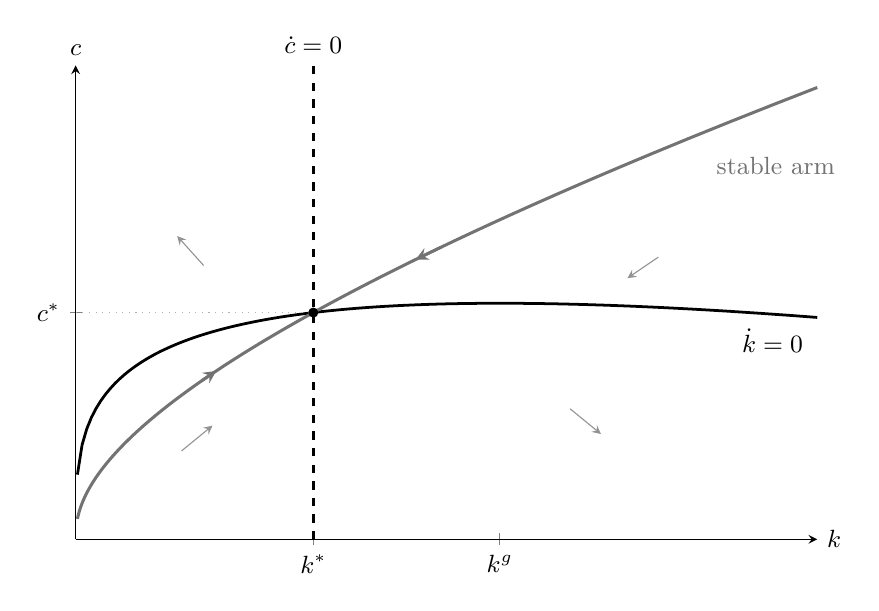
\begin{tikzpicture}
	\begin{axis}[
			width=11cm, height=7.6cm,
			axis lines=left,
			xlabel={$k$}, ylabel={$c$},
			every axis x label/.style={at={(current axis.right of origin)},anchor=west},
			every axis y label/.style={at={(current axis.above origin)},anchor=south},
			xmin=0, xmax=8.4, ymin=0, ymax=2.25,
			xtick={2.6918,4.8040}, xticklabels={$k^{\ast}$,$k^{g}$},
			ytick={1.0767}, yticklabels={$c^{\ast}$},
			tick label style={font=\small},
			label style={font=\small},
			clip=false,
		]

		% ---- the locus \dot k = 0, that is c = f(k) - \delta k ----
		\addplot[line width=1pt, domain=0.02:8.4, samples=160] {x^0.3 - 0.1*x};
		\node[anchor=north east, font=\small] at (axis cs:8.35,1.045) {$\dot k=0$};

		% ---- the locus \dot c = 0, that is f'(k) = \rho + \delta ----
		\addplot[line width=1pt, dashed] coordinates {(2.6918,0) (2.6918,2.25)};
		\node[anchor=south, font=\small] at (axis cs:2.6918,2.26) {$\dot c=0$};

		% ---- guide line to the steady state ----
		\addplot[gray!60, dotted] coordinates {(0,1.0767) (2.6918,1.0767)};

		% ---- the stable manifold, computed ----
		\addplot[line width=1.1pt, black!55] table {
				0.020000 0.096977
				0.022191 0.101387
				0.024900 0.106534
				0.027929 0.111952
				0.031460 0.117892
				0.035262 0.123913
				0.039508 0.130253
				0.044247 0.136930
				0.049536 0.143964
				0.055432 0.151372
				0.062002 0.159173
				0.069628 0.167727
				0.077805 0.176399
				0.086896 0.185529
				0.096997 0.195142
				0.108216 0.205266
				0.120660 0.215922
				0.134449 0.227135
				0.149681 0.238906
				0.167189 0.251762
				0.185750 0.264724
				0.206146 0.278297
				0.228535 0.292508
				0.253055 0.307365
				0.279859 0.322884
				0.309099 0.339077
				0.342279 0.356655
				0.376980 0.374259
				0.414574 0.392556
				0.455218 0.411555
				0.499012 0.431236
				0.546059 0.451585
				0.596432 0.472579
				0.652430 0.495074
				0.709714 0.517282
				0.770338 0.540008
				0.834243 0.563199
				0.901249 0.586768
				0.971145 0.610628
				1.043653 0.634680
				1.121499 0.659792
				1.198224 0.683895
				1.276326 0.707833
				1.355326 0.731489
				1.434651 0.754727
				1.513747 0.777425
				1.592066 0.799472
				1.672155 0.821608
				1.747312 0.842031
				1.820223 0.861541
				1.890527 0.880087
				1.957892 0.897627
				2.022073 0.914138
				2.082887 0.929611
				2.140222 0.944052
				2.196072 0.957989
				2.246122 0.970373
				2.292626 0.981793
				2.335634 0.992282
				2.375237 1.001881
				2.411548 1.010634
				2.444707 1.018586
				2.475999 1.026057
				2.503181 1.032520
				2.527686 1.038326
				2.549678 1.043520
				2.569328 1.048147
				2.586806 1.052253
				2.602282 1.055881
				2.616425 1.059189
				2.628311 1.061965
				2.638673 1.064381
				2.647653 1.066473
				2.655390 1.068273
				2.662012 1.069812
				2.667643 1.071120
				2.672568 1.072263
				2.676517 1.073179
				2.679793 1.073939
				2.682485 1.074563
				2.684673 1.075070
				2.686431 1.075477
				2.687825 1.075800
				2.688915 1.076052
				2.689782 1.076253
				2.690406 1.076397
				2.690866 1.076504
				2.691196 1.076580
				2.691426 1.076634
				2.691581 1.076669
				2.691680 1.076692
				2.691741 1.076706
				2.691774 1.076714
				2.691790 1.076718
				2.691797 1.076719
				2.691800 1.076720
				2.691800 1.076720
				2.691800 1.076720
				2.691801 1.076720
				2.691803 1.076721
				2.691808 1.076722
				2.691823 1.076725
				2.691851 1.076732
				2.691904 1.076744
				2.691992 1.076764
				2.692138 1.076798
				2.692351 1.076848
				2.692659 1.076919
				2.693091 1.077019
				2.693680 1.077155
				2.694466 1.077337
				2.695492 1.077574
				2.696812 1.077880
				2.698558 1.078284
				2.700664 1.078771
				2.703264 1.079372
				2.706441 1.080106
				2.710286 1.080994
				2.714898 1.082059
				2.720391 1.083326
				2.727170 1.084888
				2.734849 1.086657
				2.743818 1.088721
				2.754237 1.091115
				2.766284 1.093879
				2.780146 1.097056
				2.796037 1.100690
				2.814964 1.105009
				2.835723 1.109735
				2.859274 1.115083
				2.885916 1.121114
				2.915978 1.127897
				2.949813 1.135503
				2.987818 1.144012
				3.032234 1.153910
				3.080125 1.164527
				3.133631 1.176324
				3.193325 1.189406
				3.259837 1.203887
				3.333851 1.219886
				3.416136 1.237534
				3.511390 1.257790
				3.613229 1.279247
				3.726153 1.302810
				3.851284 1.328649
				3.989854 1.356947
				4.143206 1.387896
				4.312842 1.421706
				4.500403 1.458599
				4.716419 1.500491
				4.946328 1.544419
				5.200231 1.592197
				5.480543 1.644113
				5.789903 1.700472
				6.131251 1.761604
				6.507805 1.827863
				6.940567 1.902614
				7.400274 1.980527
				7.907069 2.064798
				8.400000 2.145277
			};
		\node[anchor=north west, font=\small, black!55] at (axis cs:7.15,1.86)
		{stable arm};

		% ---- steady state ----
		\filldraw (axis cs:2.6918,1.0767) circle (1.6pt);

		% ---- directional arrows in the four regions ----
		\draw[->,>=stealth,gray!85] (axis cs:1.45,1.30) -- (axis cs:1.15,1.44);
		\draw[->,>=stealth,gray!85] (axis cs:1.20,0.42) -- (axis cs:1.55,0.54);
		\draw[->,>=stealth,gray!85] (axis cs:6.60,1.34) -- (axis cs:6.25,1.24);
		\draw[->,>=stealth,gray!85] (axis cs:5.60,0.62) -- (axis cs:5.95,0.50);

		% ---- arrows along the stable arm, pointing towards the steady state ----
		\draw[->,>=stealth,black!55,line width=1pt]
		(axis cs:1.434651,0.754727) -- (axis cs:1.592066,0.799472);
		\draw[->,>=stealth,black!55,line width=1pt]
		(axis cs:4.143206,1.387896) -- (axis cs:3.851284,1.328649);
	\end{axis}
\end{tikzpicture}
